\chapter{Estimating the luminosity}\label{chap:luminosity}

%\epigraph{As for their appearance, the four of them looked alike; each was like a wheel intersecting a wheel. Their entire bodies, including their backs, their hands and their wings, were completely full of eyes, as were their four wheels.}{Ezekiel,10:10-12}
\section{Concept of luminosity}
In particle physics experiments, the energy available for producing new effects is a crucial parameter. This energy is determined by the centre of mass energy, which can be optimized through colliding beams, minimizing energy loss in the motion of the centre of mass system. Another critical aspect is the number of useful interactions or events, especially when studying rare events with a small production cross-section $\sigma_p$. The ability of a particle accelerator to produce the required number of interactions is quantified by the concept of luminosity, defined as the proportionality factor between the number of events per second $\tfrac{dR}{dt}$ and the cross-section. The relation between luminosity $\mathcal{L}$, cross-section $\sigma_p$ and ratio $\tfrac{dR}{dt}$ is defined as:
\begin{equation}
    \frac{dR}{dt} = \mathcal{L}{\sigma_p}\label{lumi_def}
\end{equation}
The unit of luminosity is therefore $\SI{}{\per\centi\meter\squared\per\second}$

Equation \ref{lumi_def} can be used to indirectly estimate luminosity from a known cross section. The basic relationship between luminosity and cross section is given by:

\begin{equation}
\mu_{\text{vis}} = \frac{R_{\text{vis}}}{f} = \frac{L_{\text{inst}} \sigma_{\text{vis}}}{f}\label{mu_def}
\end{equation}

where:
\begin{itemize}
\item  $R_{\text{vis}}$ is the interaction rate of a visible process,
\item  $f$ is the frequency of collisions,
\item  $\mathcal{L}$ is the instantaneous luminosity,
\item  $\sigma_{\text{vis}}$ is the cross section of the chosen visible process, and
\item  $\mu_{\text{vis}}$ represents the average number of visible proton-proton (pp) interactions per crossing.
\end{itemize}
This relationship can be used to measure luminosity indirectly by determining \(\mu_{\text{vis}}\) from effective processes, such as those producing at least two reconstructed VELO tracks. Once \(\mu_{\text{vis}}\) is measured, the luminosity can be derived as follows:

\begin{equation}
\mathcal{L} = \frac{\mu_{\text{vis}} \cdot f}{\sigma_{\text{vis}}}
\end{equation}

This approach is referred to as ``relative luminosity determination" because it relies on a known cross section to ``calibrate" the luminosity, using it as a normalization factor. During periods of data-taking at LHCb, different ``luminosity counters" record the values of visible interactions, allowing to calculate $\mu_{\text{vis}}$. This data is then used to estimate the instantaneous luminosity, enabling accurate cross-section measurements and experimental calibration.


% Integrated Luminosity Definition
The maximum luminosity, and therefore the instantaneous number of interactions per second, is a significant factor in particle collider experiments. However, the final figure of merit is the integrated luminosity, denoted by $\mathcal{L}_{\text{int}}$. Over a given time period \(T\), it is defined as follows:

\begin{equation}
\mathcal{L}_{\text{int}} = \int_0^T \mathcal{L}(t) dt .
\end{equation}
Integrated luminosity is crucial because it directly relates with the total number of events of interest:

\begin{equation}
\mathcal{L}_{\text{int}} \times \sigma_p = \text{number of events of interest}.
\end{equation}

The unit of integrated luminosity is therefore $\SI{}{\per\centi\meter\squared}$, but more often the barn unit is used, which is defined as $\SI{1}{\barn}=\SI{1e-24}{\per\centi\meter\squared}$. The integrated luminosity is therefore the statistics used for indicating the quantity of data available for the analysis.

% Luminosity Decay Model
A key factor influencing integrated luminosity is the decay of instantaneous luminosity over time, caused by various factors like beam intensity reduction, transverse emittance growth, and bunch length increase. A common model to represent this decay assumes an exponential form:

\begin{equation}
\mathcal{L}(t) = \mathcal{L}_0 \exp\left( -\frac{t}{\tau} \right)
\end{equation}

where $\mathcal{L}_0$ is the initial luminosity, \(t\) is the elapsed time, and \(\tau\) is the lifetime associated with the decay. 

In the following subsection a theoretical description of the instantaneous luminosity concept will be given.
In the next section, I will describe the luminosity at LHCb and explain how at this experiment we can avoid the exponential decay.

\paragraph{Luminosity in Fixed Target Experiments}
In fixed target experiments, the luminosity is influenced by the properties of both the incoming beam and the stationary target. The incoming beam is characterized by its flux $\Phi$, which is the number of particles per second. The target is described by its density $\rho_T$ and its length $l$. The luminosity in this setup is calculated using the formula:

\[
\mathcal{L}_{FT} = \Phi \cdot \rho_T \cdot l
\]

Given this definition, the interaction rate can be expressed as:

\[
\frac{dR}{dt} = \Phi \cdot \rho_T \cdot l \cdot \sigma_p
\]

\paragraph{Luminosity in Colliding Beam Experiments}
In colliding beam experiments, both beams act as the target and the incoming beam simultaneously. The general expression for luminosity in this case involves the convolution of the 3-D distribution functions of the beams, considering the overlap integral. A schematic picture is shown in Figure \ref{fig:lumi-def}\cite{Herr:941318}. Since the two beams are not stationary but moving through each other, the overlap integral depends on the longitudinal position of the bunches and therefore on the time as they move towards and through each other. For our integration we use the distance of the two beams to the central collision point $s_0 = ct$ as the ”time” variable. 
The luminosity is proportional to the overlap integral of the two  $\rho_1$, $\rho_2$ time dependent beam density distribution function:

\begin{figure}
    \centering
    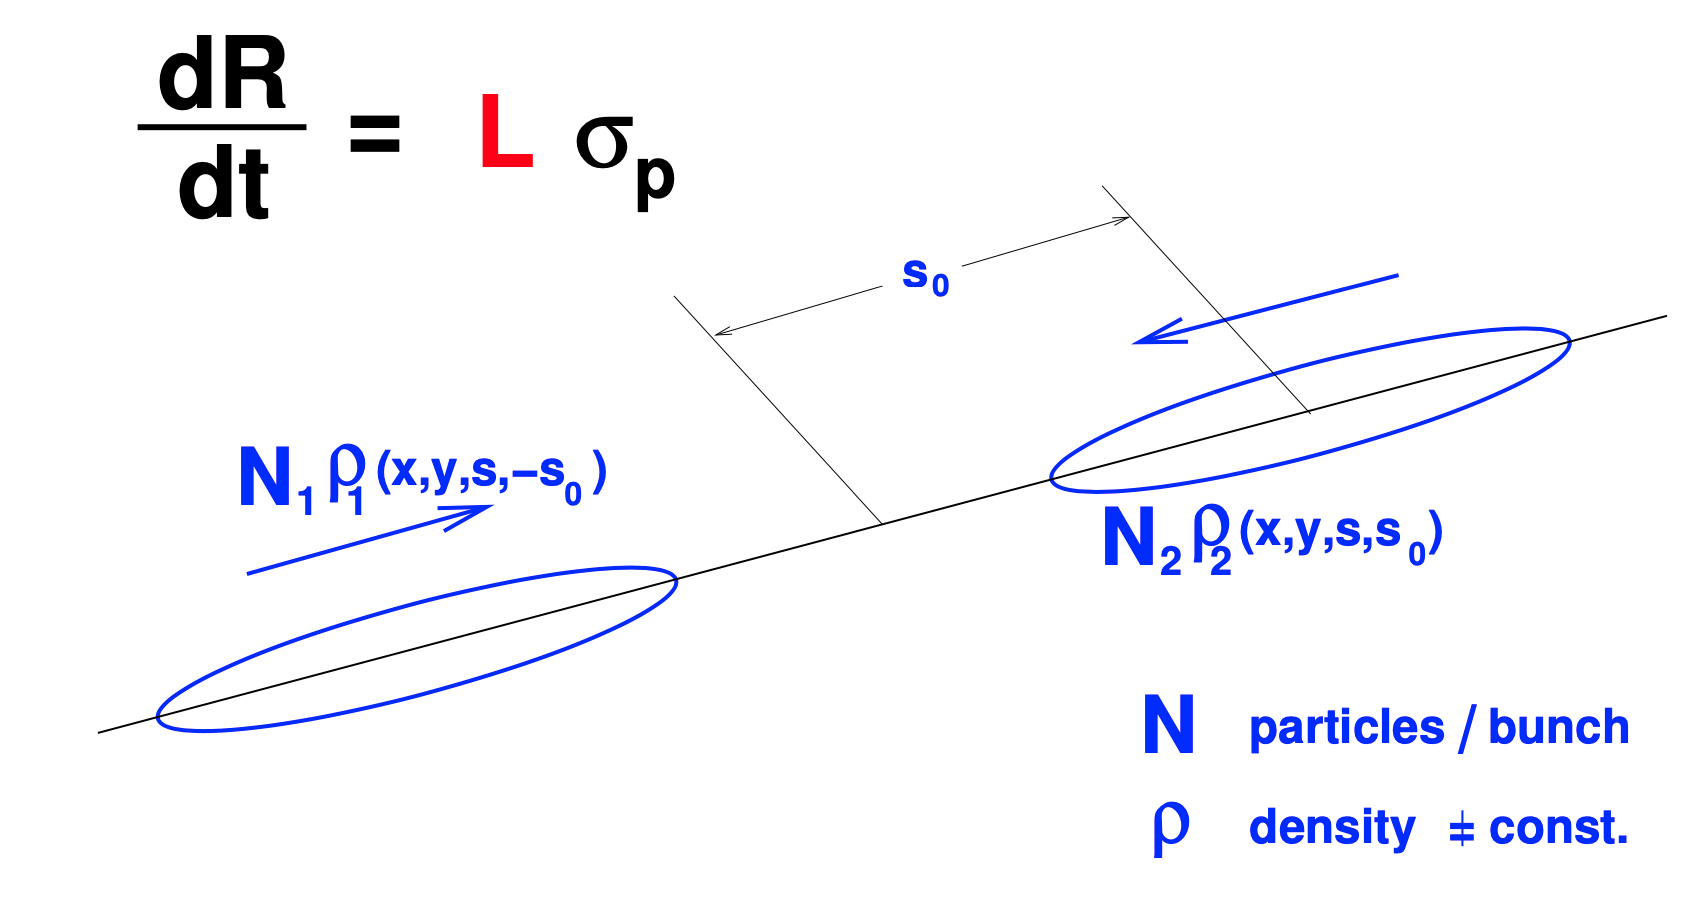
\includegraphics[width=0.6\textwidth]{figures/luminosity_def.png}
    \caption{Schematic view of a colliding beam interaction.}
    \label{fig:lumi-def}
\end{figure}

\begin{equation}
    \mathcal{L} \propto K\cdot\iiiint_{-\infty}^{+\infty}\rho_1(x,y,s,s_0)\rho_2(x,y,s,s_0)dxdydsds_0.\label{lumi_propto}
\end{equation}

Assuming colliding bunches moving against each other that meet at $s_0$, we have to take into account the kinematic factor\cite{Moller}:
\begin{equation}
    K = \sqrt{\bigl(\vec{v_1}-\vec{v_2}\bigr)^2-\bigl(\vec{v_1} \times \vec{v_2}\bigr)^2/c^2}.
\end{equation}
By further assuming head-on collisions ($\vec{v_1}=-\vec{v_2}$) and that all densities are uncorrelated in all planes, we can write:
\begin{equation}
        \mathcal{L} = 2 N_1 N_2 f N_b\cdot\iiiint_{\infty}^{+\infty}\rho_{1x}(x)\rho_{1y}(y)\rho_{1s}(s+s_0)\rho_{2x}(x)\rho_{2y}(y)\rho_{2s}(s+s_0)dxdydsds_0.\label{beam_overlap}
\end{equation}

where:
\begin{itemize}
    \item \( N_1 \) and \( N_2 \) are the number of particles per bunch for each beam;
    \item \( f \) is the revolution frequency;
    \item \( N_b \) is the number of bunches in each beam.
\end{itemize}

To evaluate this integral one should know all distributions. An analytical calculation is not always possible and a numerical integration may be required. However in many cases the beams follow ``reasonable” profiles and we can obtain closed solutions. It is often assumed that the beam profiles follow Gaussian distributions. This assumption is justified because the luminosity is determined by the overlap of the core of the distributions, with the tails contributing minimally.
Given Gaussian profiles, we can write the distribution function for a Gaussian beam in a general form:
\begin{equation}
\rho_{iz}(z) =\frac{1}{\sigma_{iz}\sqrt{2\pi}} \exp\left( -\frac{iz^2}{2 \sigma_{iz}^2} \right) \text{ where } i=1,2, \quad z=x,y
\end{equation}
\begin{equation}
\rho_{s}(s\pm s_0) =\frac{1}{\sigma_s\sqrt{2\pi}} \exp\left( -\frac{(s\pm s_0)^2}{2 \sigma_s^2} \right)
\end{equation}

Let's assume equal beams, i.e.  $\sigma_{iz} = \sigma_{jz}$ for $i=j$, z=$x,y,s$ and that the number of particles per bunch (\( N_1 \) and \( N_2 \)), revolution frequency (\( f \)), and number of bunches (\( N_b \)) are known. For exactly head-on collisions, in the relativistic limit the kinematic factor becomes 2.

Using this information, the integral for luminosity can be derived by first considering the overlap integral of the Gaussian distributions as in equation \eqref{beam_overlap}:

\begin{equation}
\mathcal{L} = \frac{2  N_1 N_2 f N_b}{(\sqrt{2\pi})^6 \sigma_x^2\sigma_y^2\sigma_s^2}\iiiint e^{-\frac{x^2}{ \sigma_x^2}} e^{-\frac{y^2}{\sigma_y^2}} e^{-\frac{s^2}{\sigma_s^2}}e^{-\frac{s_0^2}{\sigma_s^2}}dxdydsds_0.
\end{equation}

After integrating over $s$ and $s_0$\footnote{Gassuain integral: $\int_{-\infty}^{+\infty}e^{-at^2}dt = \sqrt{\tfrac{\pi}{a}}$}, we get a first intermediate result:
\begin{equation}
    \mathcal{L} = \frac{2  N_1 N_2 f N_b}{8(\sqrt{\pi})^4 \sigma_x^2\sigma_y^2}\iint \exp\left(-\frac{x^2}{\sigma_x^2}\right) \exp\left(-\frac{y^2}{\sigma_y^2}\right) dxdy .\label{spec_lumi_gaus}
\end{equation}

Finally, after integration over x and y, we get the well-known formula of luminosity for colliding Gaussian beams with head-on collisions:

\begin{equation}
\mathcal{L} = \frac{N_1  N_2  f N_b}{4 \pi  \sigma_x \sigma_y}.
\end{equation}

%If we generalize to the case where the x and y beam profiles are unequal but still assume approximately equal bunch lengths (\( \sigma_{1s} \approx \sigma_{2s} \)), we get a modified formula for luminosity:

%\begin{equation}
%\mathcal{L} = \frac{N_1  N_2  f  N_b}{2 \pi \sqrt{(\sigma_{1x}^2 + \sigma_{2x}^2)(\sigma_{1y}^2 + \sigma_{2y}^2)}}.
%\end{equation}


\section{An absolute luminosity calibration: The Van der Meer scan}
The Van der Meer (VdM) method is a foundational technique used in particle physics to measure the absolute luminosity at an accelerator. It involves separating beams in the transverse plane and measuring the average number of interactions between two colliding bunches. 
Rewriting \ref{spec_lumi_gaus} for a case of two general distribution $\rho_{1,2} (x,y)$
\begin{equation}
    \mathcal{L} = N_1 N_2 f N_b\iint \rho_1(x,y) \rho_2(x,y) dxdy,\label{generic_lumi}
\end{equation}

we can then combine \ref{generic_lumi} and \ref{mu_def} in order to write the average number of interactions $\mu$  with the cross section $\sigma$ normalized by the number of particles:

\begin{equation}
\frac{\mu (\Delta x,\, \Delta y)}{N_1N_2} = \frac{\sigma}{f} \frac{\mathcal{L}}{N_1N_2} = \sigma N_b \iint \rho _1(x_2 + \Delta x,\, y_2 + \Delta y) \rho _2(x_2,y_2) dx_2\, dy_2, \label{vdm_1}
\end{equation}
where the subscript 2 of the coordinates $x_2$, $y_2$ refers to the stationary second beam, $\mathcal{L}$ is the integrated luminosity and are $\rho_{1,2}(x,y)$ the normalized transverse particle densities of the unseparated bunches when the separation in the transverse plane $\Delta x = \Delta y = 0$.

Integration over $\Delta x$ and $\Delta y$ drastically simplifies \eqref{vdm_1} since
\begin{equation} \int \rho _1(x_2 {+} \Delta x,\, y_2 {+} \Delta y) \rho _2(x_2,y_2) dx_2\, dy_2\, d\Delta x\, d\Delta y {=} 1, \label{vdm_2} \end{equation}
as can be easily proved by substituting $x_1=x_2+\Delta x,\ y_1=y_2+\Delta y$. In the new variables the integrals $\iint \rho _1(x_1,\, y_1)dx_1\,dy_1$ and $\iint \rho _2(x_2,\, y_2)dx_2\,dy_2$ decouple and reduce to unity by definition.

From \eqref{vdm_1} and \eqref{vdm_2} we obtain the VdM formula:
\begin{equation}
     \sigma = \frac{1}{N_b} \iint \frac{\mu (\Delta x,\, \Delta y)}{N_1N_2} d\Delta x\, d\Delta y= \iint \mu_{sp}d\Delta x\, d \Delta y \label{sigma_vdm}
    \end{equation}

where we defined the specific number of interactions
\begin{equation}
\mu_{sp}=\frac{\mu}{N_1 N_2}\frac{1}{N_b}.\label{mu_sp}
\end{equation}

The derivation of \eqref{sigma_vdm} uses only $\mu _{sp}$ but not $\mu$ or $N_{1,2}$ separately. Therefore, it remains valid even if $\mu$ and $N_1N_2$ change arbitrarily but proportionally during the scan, e.g. due to a gradual decrease of beam currents with time. It is required, however, that $\rho_{1,2}$ remain constant.

Achieving precise parallel translations of particle beams in the transverse plane requires complex configurations of magnets. To translate a single beam in one direction, four magnets are needed, positioned at the corners of a trapezoid-shaped trajectory. Consequently, for steering two beams in both transverse directions, a total of 16 magnets are necessary at each interaction point. Given this complexity, ensuring consistent and synchronized movement of all magnets becomes challenging.

Due to these synchronization difficulties, continuous scans are generally avoided in favor of a stepwise approach. At the LHC, for example, the specific interaction rate $\mu_{sp}(\Delta x,\Delta y)$ is measured at predefined discrete points. This step-by-step method allows for interpolation or fitting to a specific function to derive the final integral. As beams are moved from one point to another, the process waits until the slowest magnet reaches its designated current value before starting the luminosity measurement.

The stepwise scanning technique originated with Van der Meer, who invented it over 50 years ago for the Intersecting Storage Rings (ISR) accelerator\cite{Carboni:156499}. Since then, it has been successfully applied with variations at other major accelerators\cite{Rubbia:1025746}, including the LHC. The method's accuracy can range from 0.7\% to a few percent, establishing it as a reliable approach for luminosity calibration.

Despite its success in hadron colliders, the Van der Meer method can face challenges in electron-positron colliders due to strong beam–beam interactions. In these environments, luminosity is typically measured indirectly through Bhabha scattering events, where the quantum electrodynamics cross-section is well understood. In contrast, in hadron colliders, such as the LHC, it is harder to identify processes with accurately predicted cross-sections. Thus, in hadron accelerators, the best accuracy is typically achieved by directly measuring luminosity, following its definition.

In accelerator physics, it's common for particle beams to oscillate in the transverse plane due to beam optics elements designed to keep particles on a stable trajectory. These oscillations can be modeled as a combination of movements along two independent axes, x and y. As a result, the density profiles \(\rho _{1,2}(x, y)\) can often be factorized into x and y components:

\begin{equation}
\rho _{1,2}(x, y) = \rho _{1,2}^x(x) \cdot \rho _{1,2}^y(y).
\end{equation}

This factorization is critical for simplifying the calibration process, particularly when measuring luminosity. It allows the specific interaction rate \(\mu_{sp}(\Delta x, \Delta y)\) to be similarly factorized:

\begin{equation}
\mu _{sp}(\Delta x, \Delta y) = \mu ^x_{sp}(\Delta x) \cdot \mu ^y_{sp}(\Delta y).
\end{equation}

Given this factorization, the overlap integral becomes easier to calculate by reducing it to a product of one-dimensional integrals  along the lines $\Delta x = \Delta x_0$, $\Delta y = \Delta y_0$:
\begin{equation}
\sigma = \frac{\int \mu _{sp}(\Delta x, \Delta y_0)\, d\Delta x \times \int \mu _{sp}(\Delta x_0, \Delta y)\, d\Delta y}{\mu _{sp}(\Delta x_0, \Delta y_0)}.\label{definition_sigma_vdm}
\end{equation}
The integrals in the enumerator can be measured in two one-dimensional scans over $\Delta x$ at fixed $\Delta y_0$ and vice versa. Note that the formula is valid for any point $(\Delta x_0, \Delta y_0$). It might be advantageous to choose $(\Delta x_0, \Delta y_0$) not far from the point of maximal luminosity to collect sufficient statistics of interactions. This simplification is advantageous in a large-scale accelerator like the LHC because it allows for one-dimensional scans along \(\Delta x\) and \(\Delta y\), reducing beam time and minimizing potential errors due to slow drifts in beam orbits. The bias from not scanned coordinate is minimized at the maximum of $\mu$ where the derivative of e.g. $\mu_{sp}(\Delta x_0, \Delta_y)$ on $\Delta x_0$ is zero.

While the XY factorization provides a powerful framework for simplifying luminosity calibration, it is not always perfect. Imperfections in accelerator design or other factors can lead to coupling between \(x\) and \(y\) coordinates, which may affect the accuracy of the factorization. These deviations are typically small but can introduce systematic errors in the calibration process.

To address this, the shape of the interaction vertex distributions is studied to identify any signs of non-factorizability. If the projections of the luminous region profiles onto one coordinate remain invariant when scanning the other, the factorization assumption holds. Otherwise, systematic corrections are required.

\sloppy The best way to further improve accuracy is to perform two-dimensional scans, focusing on the central region where the majority of interactions occur. This approach was pioneered at LHCb in 2017 and can significantly reduce non-factorization systematics and improve calibration accuracy\cite{Balagura_2021}.

Currently, at LHCb both in mono-directional and 2 dimensional scans are performed. First, a symmetric scan in X is performed, then a symmetric one in y and finally the 2D dimensional scan are executed. An exemple of the steps performed in the VdM scan is reported in Figure \ref{fig:vdm_steps_xy}, where is clearly visible the Turtle or Cherubin-like shape, hence the colloquial name ``turtle scan".

\begin{figure}
    \centering
    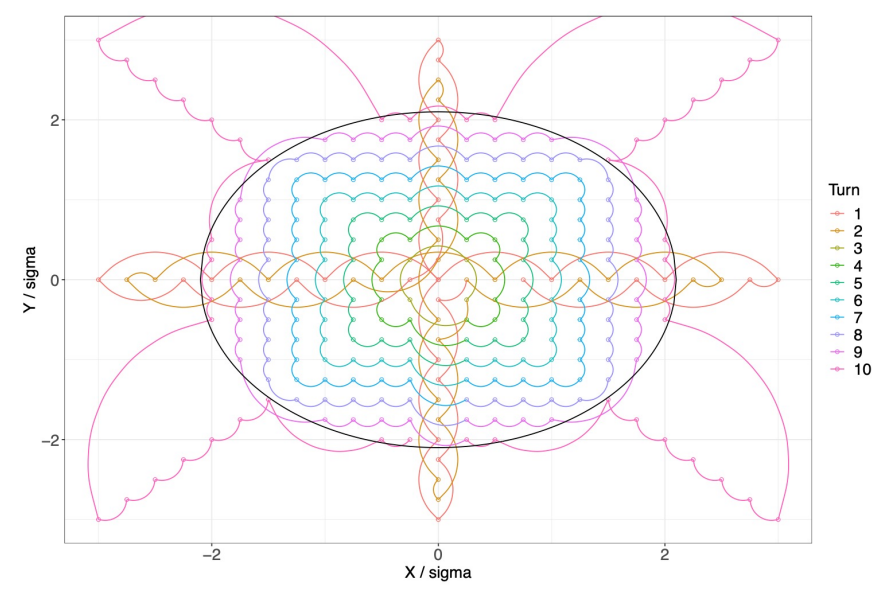
\includegraphics[width=0.7\textwidth]{figures/vdm_steps_xy.png}
    \caption{The displacement in x-y directions to perform a complete 2D Van der Meer scan.}
    \label{fig:vdm_steps_xy}
\end{figure}



\section{Luminosity at LHCb}
In late 2009, LHCb recorded its first proton-proton (pp) collisions at an injection energy of $\sqrt{s}=\SI{0.9}{\tera\eV}$. These data were used to finalize the commissioning of the sub-detector systems, calibration, and the alignment of tracking, calorimeter, and particle identification (PID) systems. During this period, the VELO was left in the open position to accommodate the larger aperture required at lower beam energies.
The operating conditions changed rapidly in 2010 due to the LHC ramp-up in luminosity. A critical parameter for LHCb performance is the pile-up \(\mu_{\text{vis}}\), defined in Eq. \ref{mu_def} as the average number of visible interactions per beam-beam crossing. Luminosities started around $\sim \SI{1e28}{\per\centi\meter\squared\per\second}$ with almost no pile-up but eventually reached $\sim \SI{1e32}{\per\centi\meter\squared\per\second}$ with $\mu_{\text{vis}} \approx 2.5$.
While the highest luminosity in 2010 was already 75\% of the LHCb design luminosity, the pile-up was much larger due to the low number of bunches in the machine. Despite this, the trigger and reconstruction systems demonstrated efficient performance under these conditions\cite{det_perf}.

%\begin{figure}
%    \centering
%    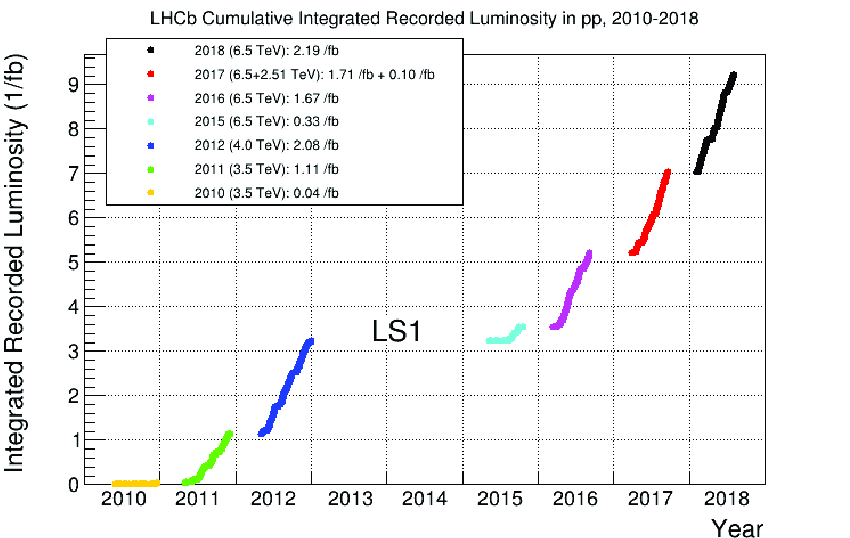
\includegraphics[width=\textwidth]{figures/lumiRun2.png}
%    \caption{Integrated luminosity during Run1 and Run2, interspersed by the LS1.}
%    \label{fig:lumiRun1Run2}
%\end{figure}

The LHC beam energy was 3.5 TeV during 2010 and 2011. In 2011, the number of bunches in the machine increased to about 1300, allowing for a reduction in pile-up while LHCb operated at a luminosity of $\SI{3.5e32}{\per\centi\meter\squared\per\second}$. This was 1.75 times the design luminosity of $\sim \SI{2e32}{\per\centi\meter\squared\per\second}$. The instantaneous luminosity directly delivered by the LHC was too high with respect to the target luminosity the LHCb experiment has been designed for, since of the too high event rate and irradiation dose to which the detectors would be subjected. Since of the higher detector hits multiplicity, track and vertex reconstructions would suffer of high event pile-up, that increases combinatorial background and complicates track reconstruction.
To cope with this issue, in 2011 the LHCb experiment introduced a luminosity levelling procedure at the LHCb interaction point to keep the instantaneous luminosity stable within about 5\% during a fill. This was achieved by adjusting the transverse overlap of the beams. For one particularly long fill, a maximum overlap with head-on beams was reached only after 15 hours. This levelling minimized the effects of luminosity decay and allowed LHCb to maintain a consistent trigger configuration, reducing systematic uncertainties due to changing detector occupancy.

In 2012, the LHC beam energy was increased to $\SI{4}{\tera\eV}$, and LHCb took data at a luminosity of $\sim \SI{4e32}{\per\centi\meter\squared\per\second}$, twice the LHCb design luminosity. An effort was made in 2012 to use more efficiently the processing power available in the Event-Filter-Farm (EFF) in order to cope with the increase in luminosity, allowing LHCb to increase the data sample available for physics analysis. This value of luminosity was kept as target until the end of Run2. 


For Run3, LHCb plan to further increase this value by 5, reaching an instantaneous luminosity of $\SI{2e33}{\per\centi\meter\squared\per\second}$
%An overview of the luminosity integrated until the end of Run 2 is depicted in Figure \ref{fig:lumiRun1Run2}.

\subsection{Luminosity leveling}\label{sec:lumi_levelling}

\begin{figure}
    \centering
    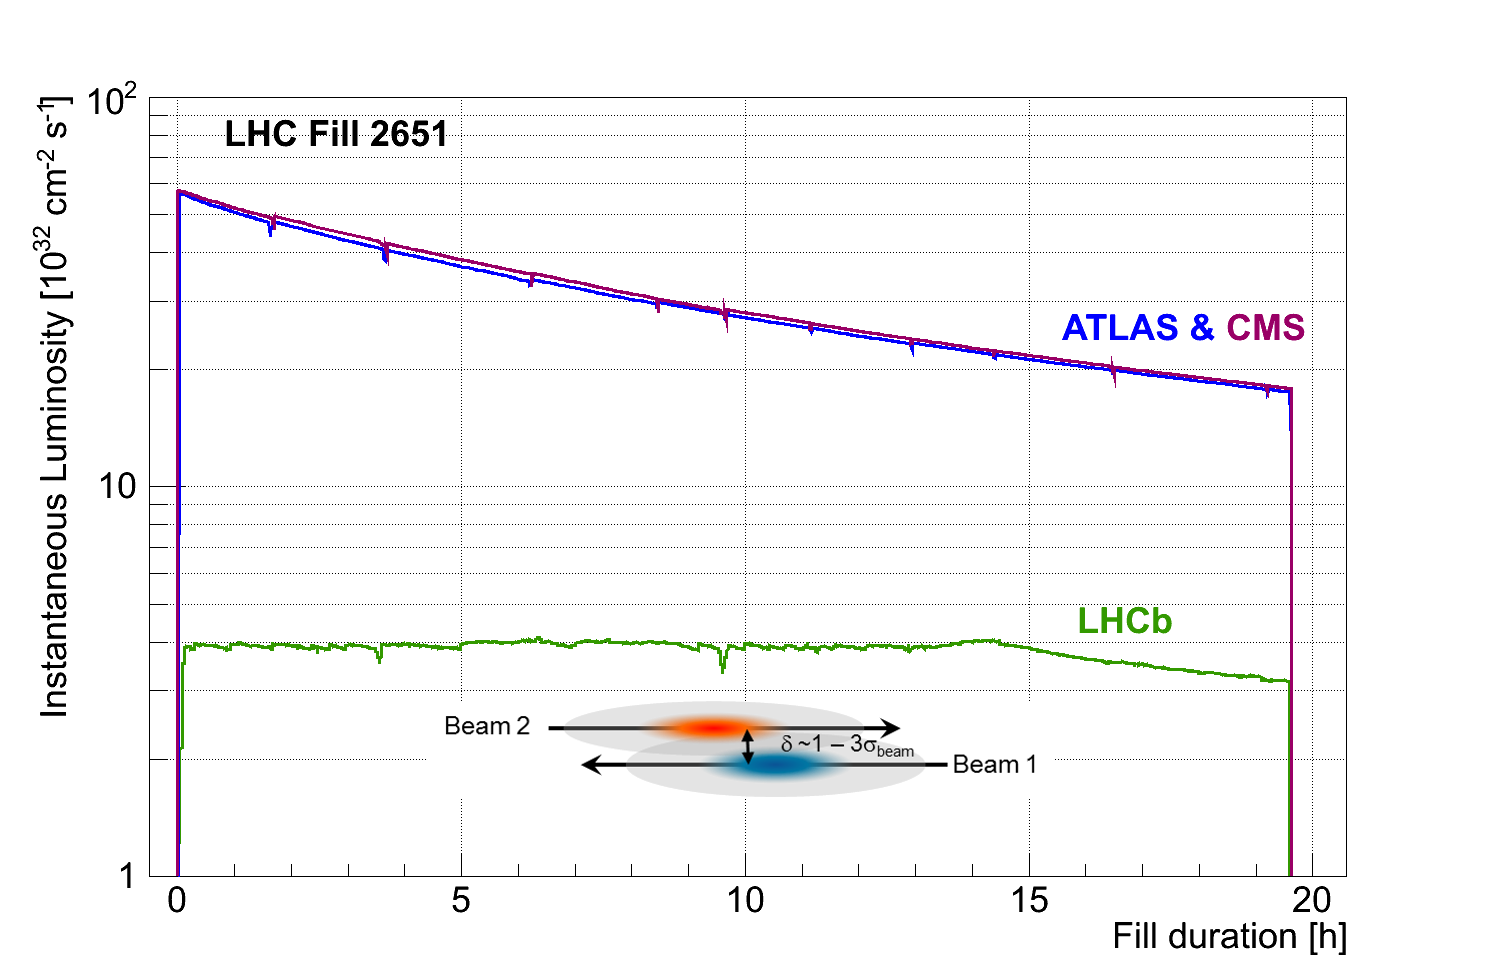
\includegraphics[width=\textwidth]{figures/luminosity_leveling.png}
    \caption{Development of the instantaneous luminosity for ATLAS, CMS and LHCb during LHC fill 2651. After ramping to the desired value of $\SI{4e32}{\per\centi\meter\squared\per\second}$ for LHCb, the luminosity is kept stable in a range of 5\% for about 15 hours by adjusting the transversal beam overlap.
    The difference in luminosity towards the end of the fill between ATLAS, CMS and LHCb is due to the difference in the final focusing at the collision points, commonly referred to as the beta function $\beta*$}
    \label{fig:lumi-leveling}
\end{figure}

Luminosity levelling is a critical technique used by the LHCb experiment to stabilize the instantaneous luminosity and control pile-up at the experiment's interaction point. It addresses the issue of excessively high event rates and irradiation doses caused by the high luminosity delivered by the LHC, which can complicate track reconstruction and increase systematic uncertainties.
The instantaneous luminosity in the LHCb experiment is kept constant at a lower value compared to other LHC experiments like CMS and ATLAS. Generally, the luminosity in an LHC fill follows an exponential decay trend due to beam intensity degradation effects. However, by using luminosity levelling, LHCb maintains the luminosity at a fixed peak value, allowing for consistent operational conditions for the DAQ and trigger systems.  This behaviour is well depicted in Figure \ref{fig:lumi-leveling}. Precision in the online measurement of instantaneous luminosity is vital for monitoring and luminosity levelling. The collaboration has estimated that an accuracy of less than 5\% is sufficient for this purpose. 


Luminosity levelling is achieved by adjusting the transverse overlap between the two colliding beams using corrector magnets located on each side of the experiment. The beam overlap is incrementally increased in small discrete steps as the beam intensity decreases, allowing for fine control of the luminosity. The adjustments are made through a luminosity control software, which provides feedback from the LHCb sub-detectors to the LHC Control Centre. A scheme of this software is reported in Figure \ref{fig:lumi-control}.
The LHCb luminosity control manager, part of the ECS, is a FSM driven by LHC operational modes. It monitors the instantaneous luminosity, compares it to the optimal target luminosity, and sends the levelling parameters to the LHC Lumi Levelling driver application. On the LHC side, this application uses a ``levelling algorithm" to determine the necessary adjustments in beam separation to maintain the target luminosity.

\begin{figure}
    \centering
    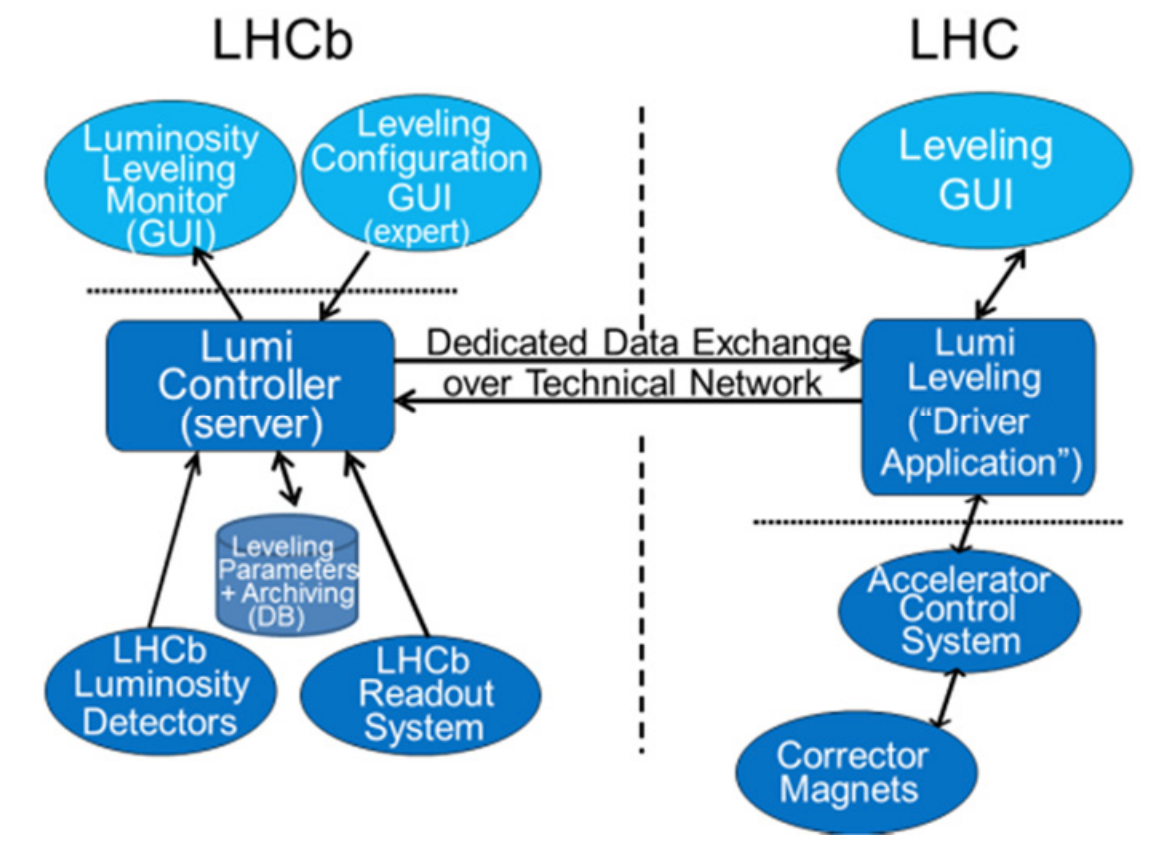
\includegraphics[width=0.8\textwidth]{figures/lumi_control.png}
    \caption{LHCb Luminosity control software diagram}
    \label{fig:lumi-control}
\end{figure}

\subsection{Luminometers}
The target luminosity for LHCb is a compromise between physics priorities, trigger selection efficiencies, detector performance limitations, DAQ system constraints, and offline data-processing capabilities. For Run-2, this value was set to $\SI{4e32}{\per\centi\meter\squared\per\second}$, while for Run-3, the optimal target luminosity is estimated at $\SI{2e33}{\per\centi\meter\squared\per\second}$, corresponding to a pile-up per bunch-crossing of approximately $\mu = 5.5$.

During Run-1 and Run-2, online luminosity estimates had a precision of 10\% and were derived from two primary sources: 
\begin{enumerate}
    \item Transverse Energy Deposition: Observations of energy depositions over a fixed threshold in the calorimeter system;
    \item Muon Station Counts: Counts in the muon stations, provided by the Level-0 (L0) hardware-trigger.
\end{enumerate}
During Run-2, the systematic uncertainty on the integrated luminosity was of 3.9\%, by far the principal source of systematics in most of the measure- ments of cross-sections (e.g. \cite{j-psi}). The aim of the collaboration for Run-3 is to increase the precision in the integrated luminosity measurement, aiming at reaching an ac- curacy of 1 − 2\%\cite{Aaij:1951625}. For this reason the collaboration decided to implement for Run-3 as many detector and systems as possible to monitor the instantaneous luminosity at the interaction point during the data-taking period.
Pile-up can be measured in various ways. One approach is to count the number of reconstructed primary vertices per event, which is directly proportional to $\mu$, up to an acceptance-efficiency factor $\epsilon$. Another method is to measure count rates, such as the number of tracks per bunch crossing, hits on a detector, or reconstructed particles. These count rates, known as luminosity counters, indirectly estimate the mean pile-up per event.

\paragraph{PLUME}
A dedicated luminometer sub-detector, PLUME (Probe for LUminosity MEasurement), was introduced for Run-3 to improve both online and offline luminosity measurement precision. PLUME consists of 24 hodoscopes (couples of detector modules read out for coincidences in both modules) surrounding the beampipe, pointing at the nominal interaction point, and located approximately 1.7 meters upstream from the collision region. It covers a high-pseudorapidity range $(2.4 < \eta < 3.1)$.

Each hodoscope module is composed of 10 × 10 × \SI{5}{\milli\meter\tothe{3}} quartz crystals, coupled with photomultipliers that detect Cherenkov light generated when high-speed particles traverse the quartz. Online luminosity measurement is performed by counting coincidences in at least one hodoscope, identifying tracks coming from the interaction region, and suppressing background activity.
In addition to the PLUME detector, LHCb introduced several other luminosity counters for online monitoring and offline luminosity measurement. This redundancy provides stability cross-checks and helps evaluate systematic uncertainties.

A problem with the luminosity linearity has been discovered in September 2022: due to non-negligible rate of random coincidences the PLUME showed divergencies from the expected linear behaviour. Since 7th of July 2022 PLUME luminosity corrected for non-linearity using HLT$1$ counters, rendering de-facto PLUME an offline luminosity estimator.


\paragraph{Other online counters} 
In addition to PLUME, there are other counters based on minimum bias conditions and independent of high-level reconstruction sequences, operating at approximately 30 MHz and read out via the ECS interface. These counters are primarily used for online monitoring and include:
\begin{itemize}
   \item VELO clusters counters based on FPGA (object of this thesis)
   \item VELO superpixel ASICS counters
   \item RICH currents counters
   \item SciFi currents counters
\end{itemize}
\paragraph{Offline counters} 
Other than online counters, there are also implemented offline counters for more precise estimates.
These counters are based on the number of reconstructed tracks, primary vertices, hits or energy deposited\
We distinguish between HLT$1$ (processed at ∼30 kHz) and HLT$2$ counters (offline).

The HLT$1$ counters include:
\begin{itemize}
   \item Number of muon hits in the muon stations (luMUONmeter).
   \item  VELO tracks in bins of $\eta$ and reconstructed primary vertices.
   \item SciFi clusters per module combinations.
   \item Energy deposition in the ECal and HCal.
\end{itemize}
The HLT$2$ counters are:
\begin{itemize}
    \item Hits in the RICH$1$ and RICH$2$ detectors.
    \item calorimeters counters after zero suppression 
\end{itemize}

\section{Online VELO Luminosity estimation}
A common method to measure luminosity in particle accelerators is through relative-luminosity measurements, which rely on the precise, event rate $\frac{dR}{dt}$ for a reference process. The basic formula, considering inelastic proton-proton (pp) processes with a cross section $\sigma_{inel}$, derives the expectation value of the instantaneous luminosity with respect to the revolution frequency, i.e. combining \eqref{lumi_def} and \eqref{mu_def}:
\begin{equation}
    \langle\mathcal{L}_{bunch}\rangle = \dfrac{\bigl<\frac{dR_{inel}}{dt}\bigr>}{\sigma_{inel}} = \langle\mu_{inel}\rangle\frac{f_{rev}}{\sigma_{inel}}
\end{equation}

The luminosity measurement can then be expressed as:
\begin{equation}
    \langle\mathcal{L}_{bunch}\rangle =  \langle\mu_{vis}\rangle\frac{f_{rev}}{\sigma_{vis}}\label{lumi_per_bunch}
\end{equation}

where $\langle\mu_{vis}\rangle$ is the visible pile-up, which can be calculated from the count rates or primary vertex measurements. The visible cross-section $\sigma_{vis}$  accounts for the acceptance-efficiency factor, with 
$\sigma_{vis} = \epsilon \sigma_{inel}$
In principle, $\langle\mu_{vis}\rangle$ is proportional to the luminosity up to a constant scale factor, enabling relative measurements. However, non-linearities can occur, particularly at high luminosity values, due to detector saturation or other factors.

Absolute luminosity measurements are possible once the visible cross-section is known, often calibrated using the Van der Meer scan, allowing for an absolute luminosity value derived from the relative measurements. In this context, the VELO cluster counters, mentioned in Section \ref{sec:velo_counters}, are employed to measure  $\langle\mu_{vis}\rangle$. This involves counting clusters $N_i$ in a defined sensor region over $N_{evt}$ events and correlating them to visible pile-up using linearity properties:
\begin{equation}
    \langle\mu_{vis}\rangle\propto \frac{\sum_i N_i}{N_{evt}}
\end{equation}

The linearity method is simple but requires linearity across the entire range of detector counts, which may not always hold, especially at high particle multiplicities. However, intensive studies were performed on Monte Carlo simulations up to a pile-up $\mu = 28$, showing perfect linearity for these luminosity counters\cite{dan}. The linear behaviour is also confirmed on collision data in several fills, such as the one depicted in Figure \ref{fig:muscan}.

\begin{figure}
    \centering
    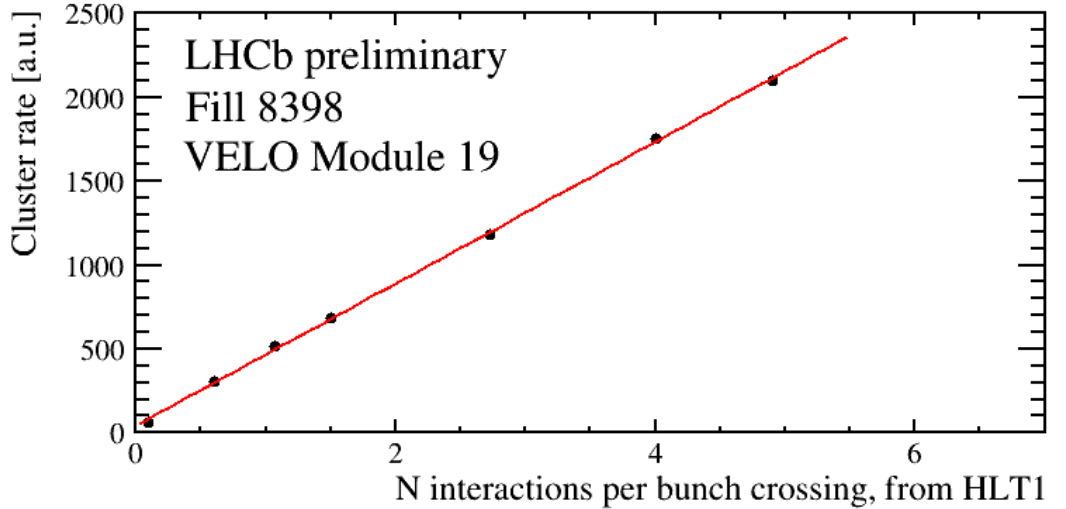
\includegraphics[width=\textwidth]{figures/muscan.png}
    \caption{Linearity of cluster counters during mu scan of November 2022}
    \label{fig:muscan}
\end{figure}


\subsection{Calibration of each counter with VdM scan}\label{sec:calibration_vdm}
Each one of the 208 cluster counters is calibrated during the VdM scan independently. To explain the process, I'll use the VdM scan conducted on September 7, 2023, as an example.
It was a full 5 hours program with two symmetric scans and two 2-dimensional scans. Two additional symmetric, 2-dimensional scans two Length Scale Calibrations (LSC) were performed with smog. Figure \ref{fig:inner_vdm_sep} provides an overview of the VdM scan setup, illustrating the raw mean counts per event for the inner counters and the x and y positions of the two beams.



\begin{figure}
    \centering
    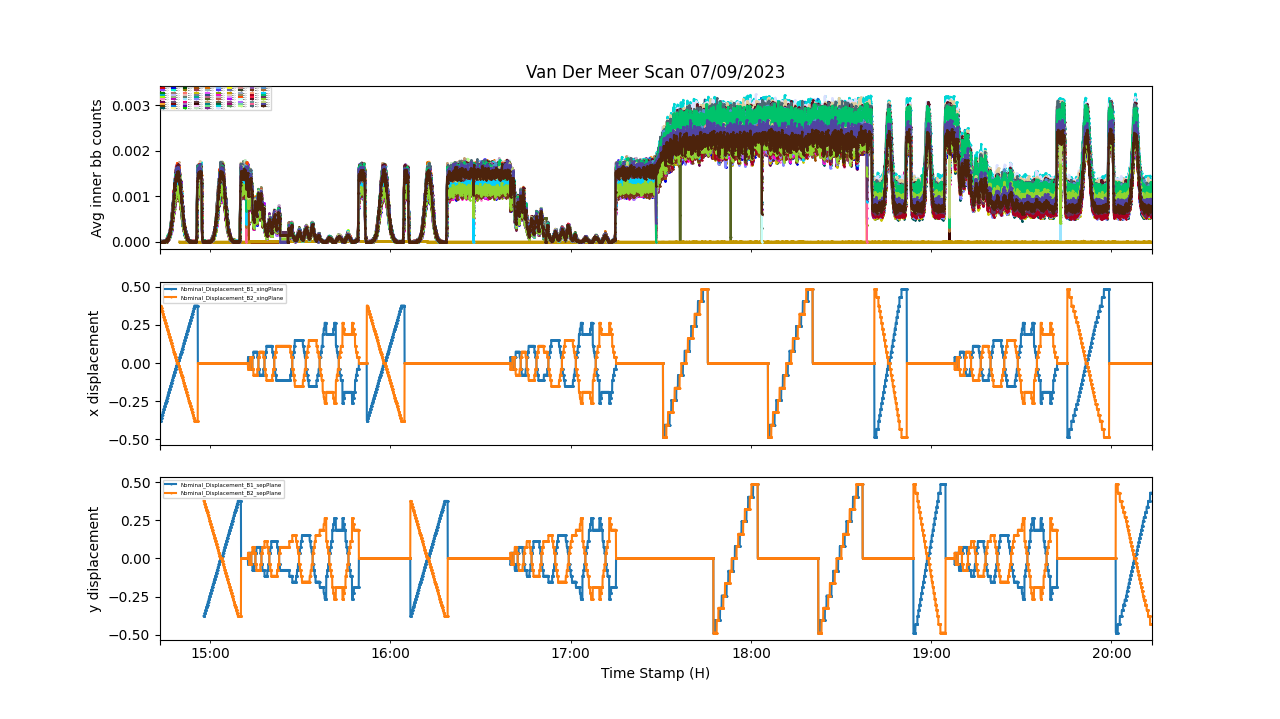
\includegraphics[width=\textwidth]{figures/inner_counts_bkg.png}
    \caption{Overview of the Van der Meer Fill of 7th September 2023. The first panel illustrates the raw mean counts per event of the 104 inner counters, while the second and third panels respectively depict the x and y positions of the two beams. Notice how an offset is introduced in the counters rate at $\approx$17:40 due to the SMOG injection.}
    \label{fig:inner_vdm_sep}
\end{figure}


During the initial phase of the scan, background noise was negligible, allowing the measurements to focus on the counts related to proton-proton (pp) interactions. However, after the SMOG injection ($\approx$17:40), the background due to collisions of proton bunches with empty bunches becomes important. As described in Section \ref{sec:velo_counters}, there are implemented 4 different counters for each bunch crossing type, allowing the subtraction of the background as an online procedure. In the calibration phase this step is perfected offline. 

Another important step in the calibration involves normalizing the counters to account for variations in the bunch population throughout the fill. This division allows for the estimation of $\mu_{sp}$ defined in \eqref{mu_sp}. This is crucial for obtaining accurate and consistent results.

Figure \ref{fig:bkg_sub_calib} shows the corrected data with the background subtracted, highlighting in a purple box the VdM steps used in the calibration. These steps are, in chronological order, a symmetric X scan, asymmetric Y scan and a 2D scan (or turtle scan). 

\begin{figure}
    \centering
    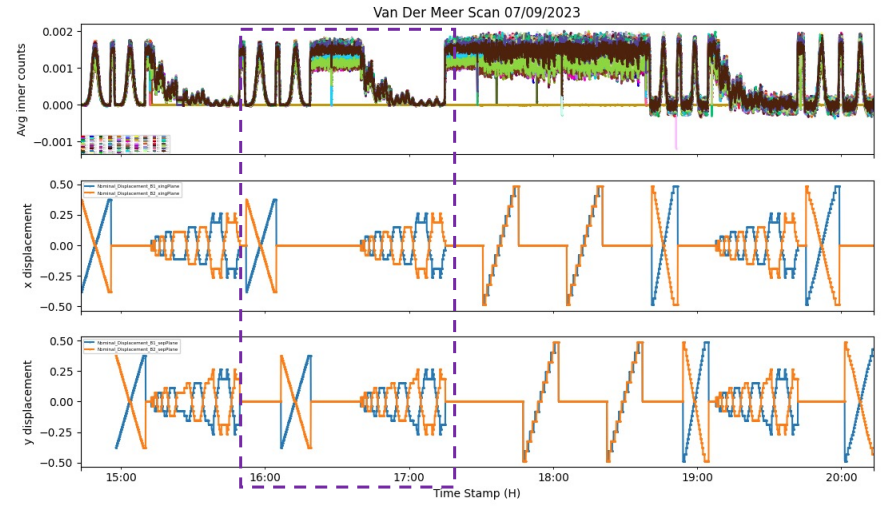
\includegraphics[width=\textwidth]{figures/calibration_period.png}
    \caption{Behaviour of the counters with subtracted background. Notice in fact how there is no more baseline after 17:40, as it were in Figure \ref{fig:inner_vdm_sep}. Additionally, the region used for the calibration is highlighted in the purple box. In this selected region a symmetric scan in X, a symmetric scan in Y and a 2D scan were performed.}
    \label{fig:bkg_sub_calib}
\end{figure}

The calibration involves fitting a 2D Gaussian to the counter data as a function of x and y displacements, as described in \eqref{sigma_vdm}. This step is necessary to establish the relationship between the observed counts and the expected Gaussian distribution, providing a means to correct for potential misalignments or shifts in the detector response. Figure \ref{fig:fit_example} illustrates an example of such a 2D Gaussian fit, along with the corresponding residuals, demonstrating how the calibration is carried out.


\begin{figure}
    \centering
    \begin{subfigure}{0.48\textwidth}
    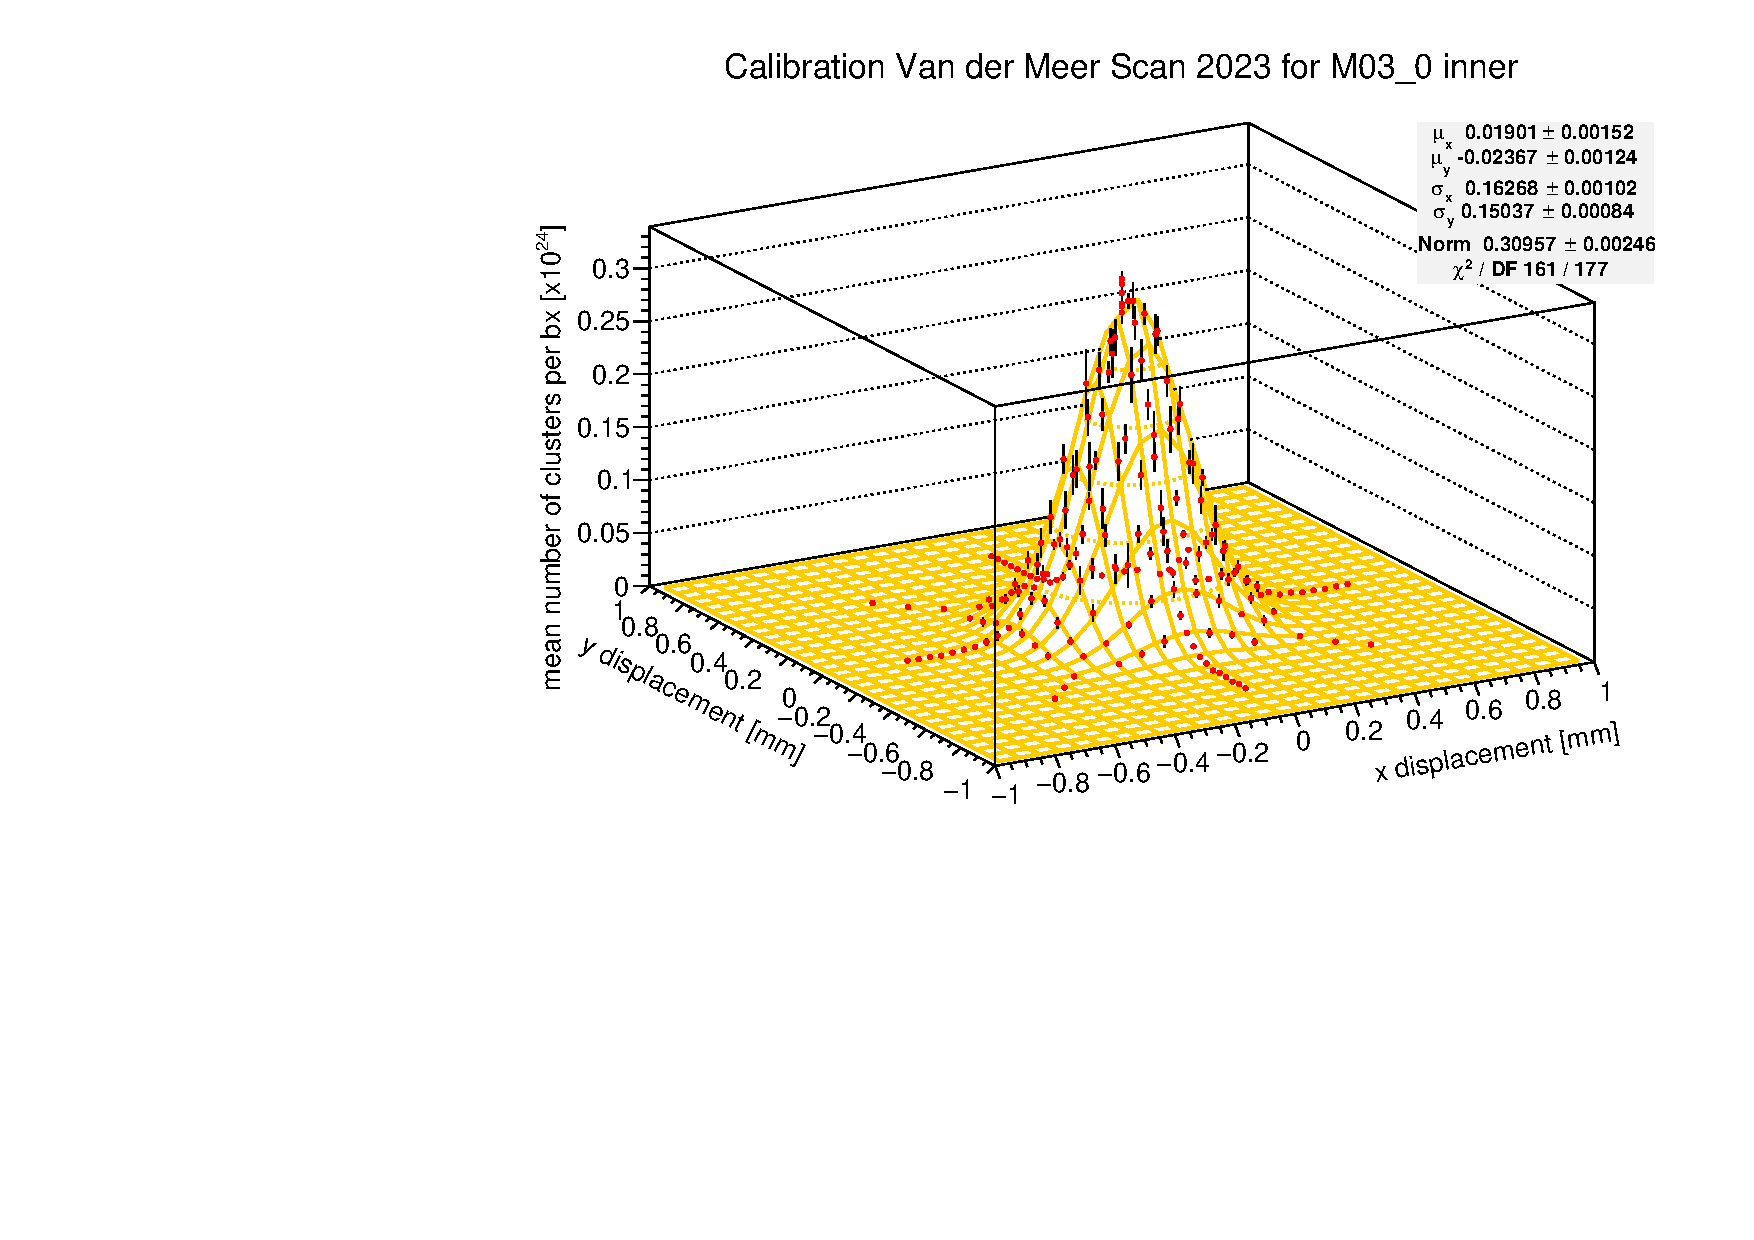
\includegraphics[width=\linewidth]{figures/M03_0.pdf}
    \caption{2D Gaussian fit to the counter M$03\_0$ inner}\label{fig:fit_M03}
    \end{subfigure}
    \begin{subfigure}{0.48\textwidth}
    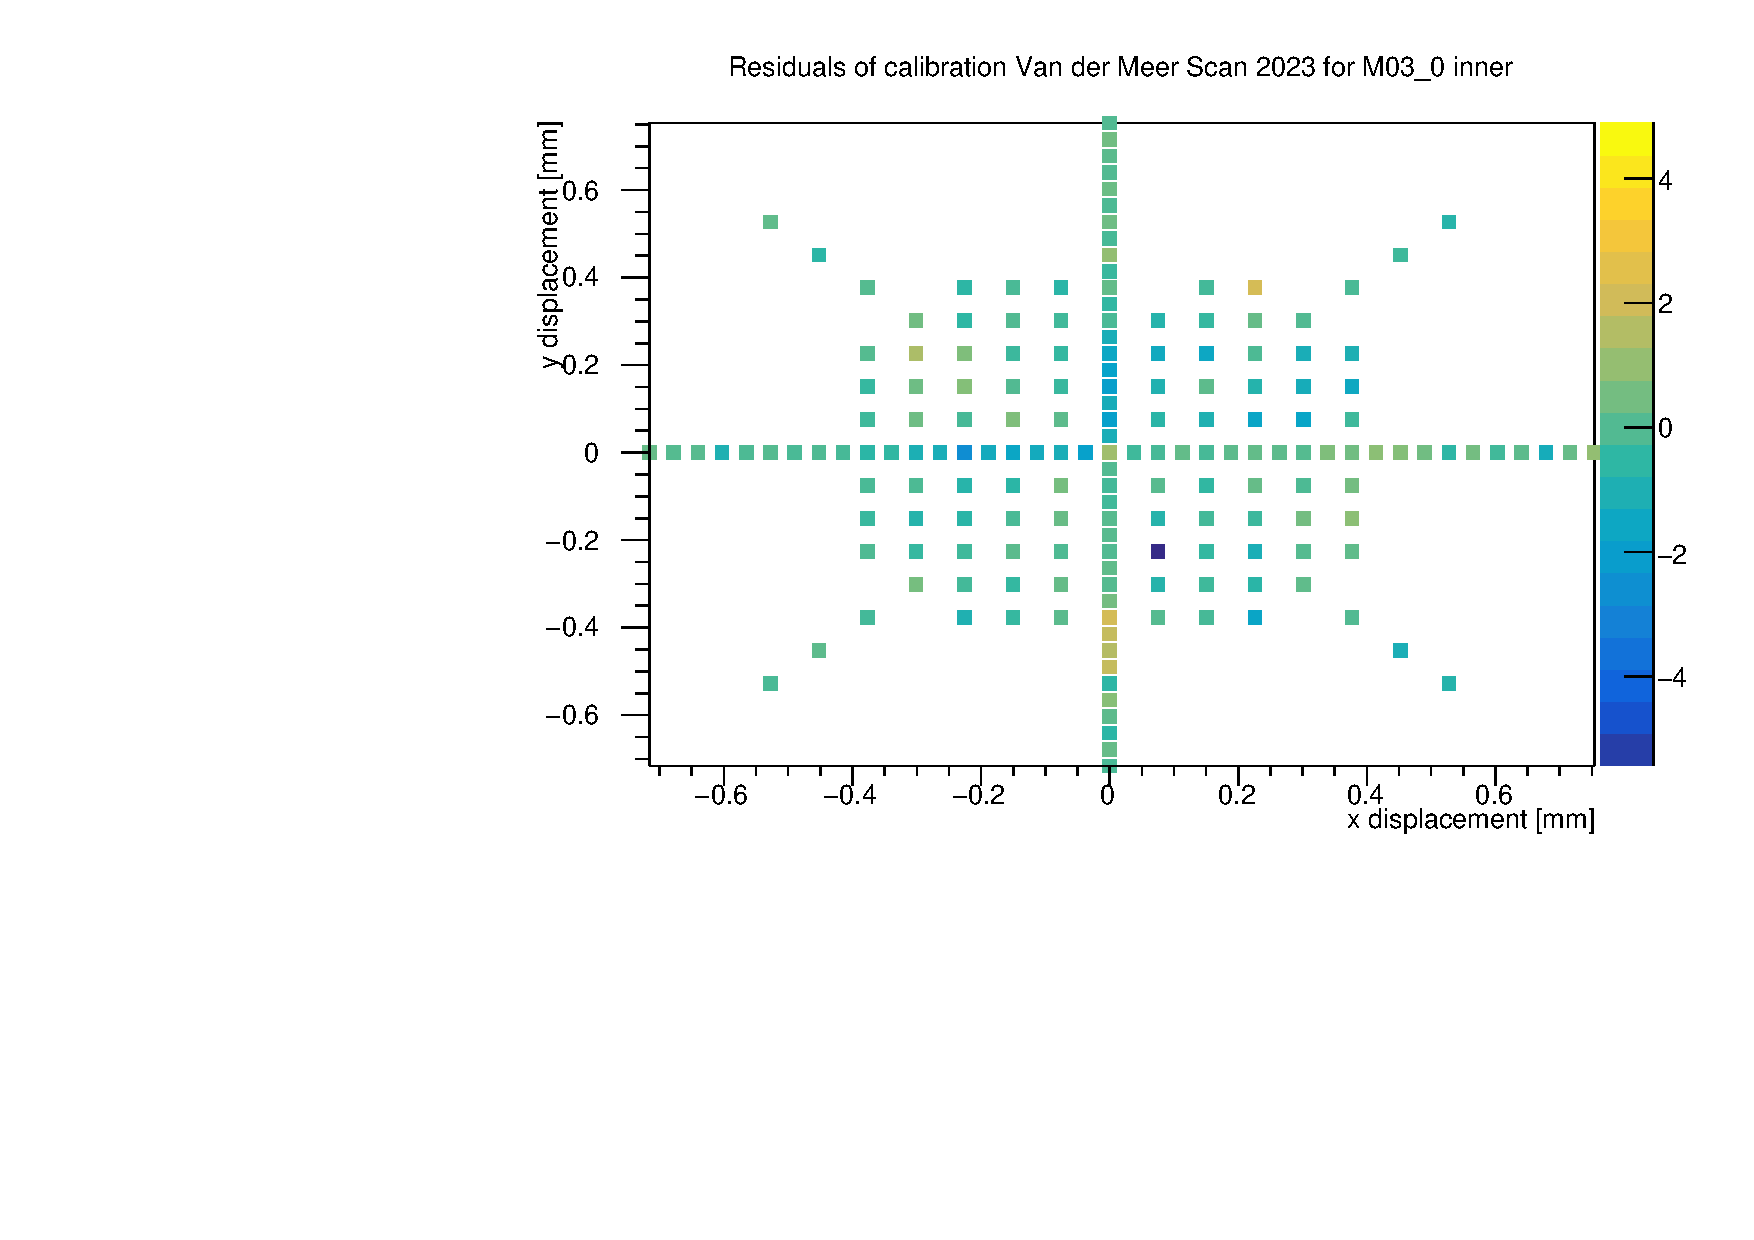
\includegraphics[width=\linewidth]{figures/M03_0_res.pdf}
    \caption{Residuals of the fit}\label{fig:M03_res}
    \end{subfigure}
    \caption{Example of a 2D Gaussian fit for performing the calibration of each counters during the Van der Meer scan}
    \label{fig:fit_example}
\end{figure}

The underlying density function for the distribution of the counts as a function of the displacements $x$ and $y$ in a bivariate Gaussian, whose analytical form is given by Equation \eqref{2d-gaus}. 
\begin{equation}
    f(x,y|\mu_{x,y},\sigma_{x,y},\rho)=\exp{\left(-{\frac {1}{2\left[1-\rho ^{2}\right]}}\left[\left({\frac {x-\mu _{X}}{\sigma _{X}}}\right)^{2}-2\rho \left({\frac {x-\mu _{X}}{\sigma _{X}}}\right)\left({\frac {y-\mu _{Y}}{\sigma _{Y}}}\right)+\left({\frac {y-\mu _{Y}}{\sigma _{Y}}}\right)^{2}\right]\right)}\label{2d-gaus}.
\end{equation}

This function describes the expected distribution of counts based on the Gaussian assumption, with key parameters such as mean $\mu$, standard deviation $\sigma$, and correlation coefficient $\rho$. To ensure proper normalization, the integral of this function is computed to obtain the normalization factor, as shown in Equation \eqref{2d-gaus-norm}. This normalization factor represents the visible cross section, $\sigma_vis$, which is the ultimate quantity to calculate for performing the calibration.

\begin{equation}
    N = 2\pi \sigma_{X}\sigma_{Y}\sqrt {1-\rho ^{2}}=\sigma_{vis}\label{2d-gaus-norm}
\end{equation}
 The results of each $\sigma_{vis}$ are reported as a function of the $z$ position of the module in Figure \ref{fig:coefficient_pos}, demonstrating how the calibration varies depending on the position along the detector's z-axis.

\begin{figure}
    \centering
    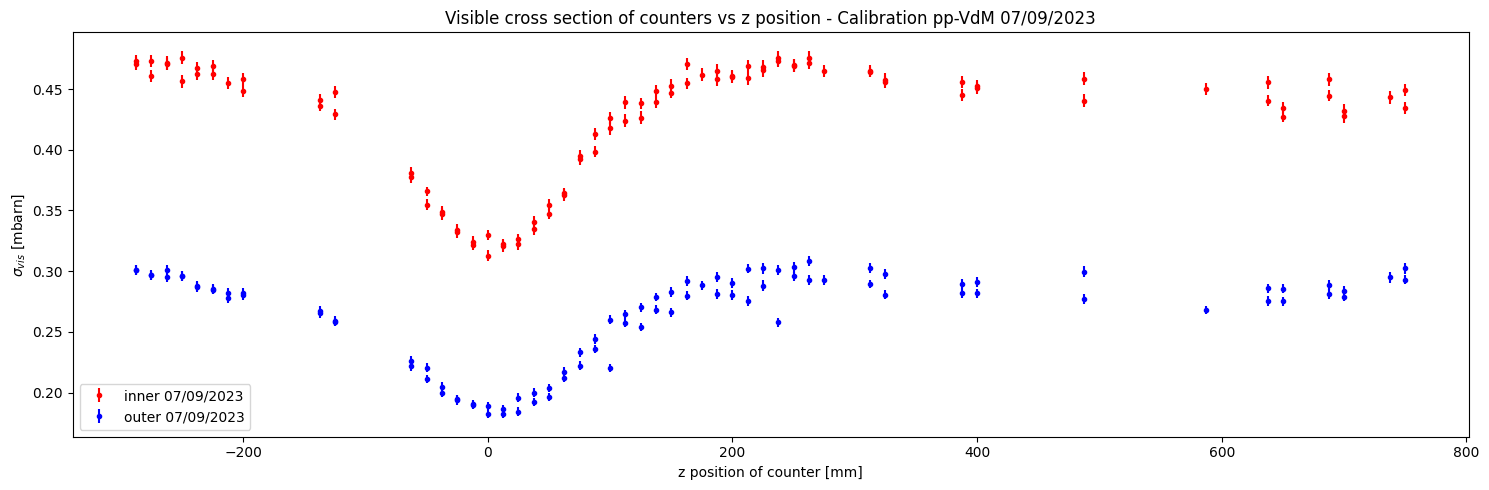
\includegraphics[width=\textwidth]{figures/coefficient_pos.png}
    \caption{Results of the $\sigma_{vis}$ for each counter, as a function of its position along the $z$-axis of the detector. The bell around $z=0$ is expected due to the VELO acceptance and confirmed in simulation.}
    \label{fig:coefficient_pos}
\end{figure}

Once every visible cross section $\sigma_{vis}$ is calculated, each one of the counters can provide a luminosity estimation based on the definition in \eqref{lumi_per_bunch}.

\subsection{Combining the counters for a single luminosity measurement}
There is now the issue on how to combine the counters for a single luminosity measurement. In fact, the calibration with the VdM scan allowed to calculate a calibration factor for every counter, leaving potentially 208 different luminosity measurements. 
First off, the question is what distribution follow all the different measurement at the same timestamp. 
The distribution of all the estimation performed during the VdM fill of 7th September 2023 is reported in Figure \ref{fig:lumi_hist_ts} at two different timestamps spaced by 15 minutes. The distribution is not Gaussian, but it has a bell shape. Therefore, we are encouraged to use mean and standard deviation as metrics to describe the peak and the width of the curve. 


\begin{figure}
    \centering
    \begin{subfigure}{0.48\textwidth}
    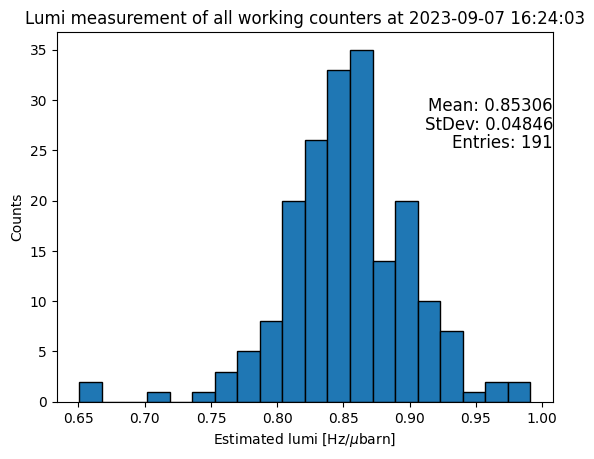
\includegraphics[width=\linewidth]{figures/lumi_hist_1624.png}
    \caption{Timestamp 16:24}\label{fig:lumi1624}
    \end{subfigure}
    \begin{subfigure}{0.48\textwidth}
    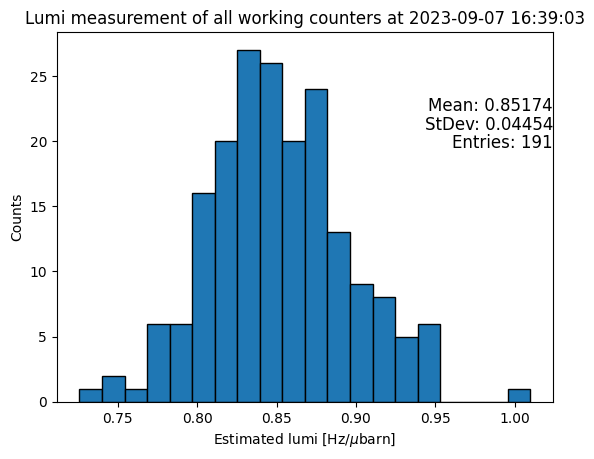
\includegraphics[width=\linewidth]{figures/lumi_hist_1639.png}
    \caption{Timestamp 16:39}\label{fig:lumi1639}
    \end{subfigure}
    \caption{Distribution of the luminosity estimation of all the working counters during the VdM scan fill of 7th September 2023. Two different timestamps are reported at a distance of 15 minutes one to the other. }
    \label{fig:lumi_hist_ts}
\end{figure}

In fact, we see in the trace plots of Figure \ref{fig:std_dev_rel_std} (left) that the standard deviation of the luminosity estimations is proportional to the luminosity estimation. This encourages us to study the relative standard deviation defined as the standard deviation $\sigma$  divided by the mean $\mu$:
\begin{equation}
    \sigma_{rel} = \frac{\sigma}{\mu} \label{rel_std}.
\end{equation}


\begin{figure}
    \centering
    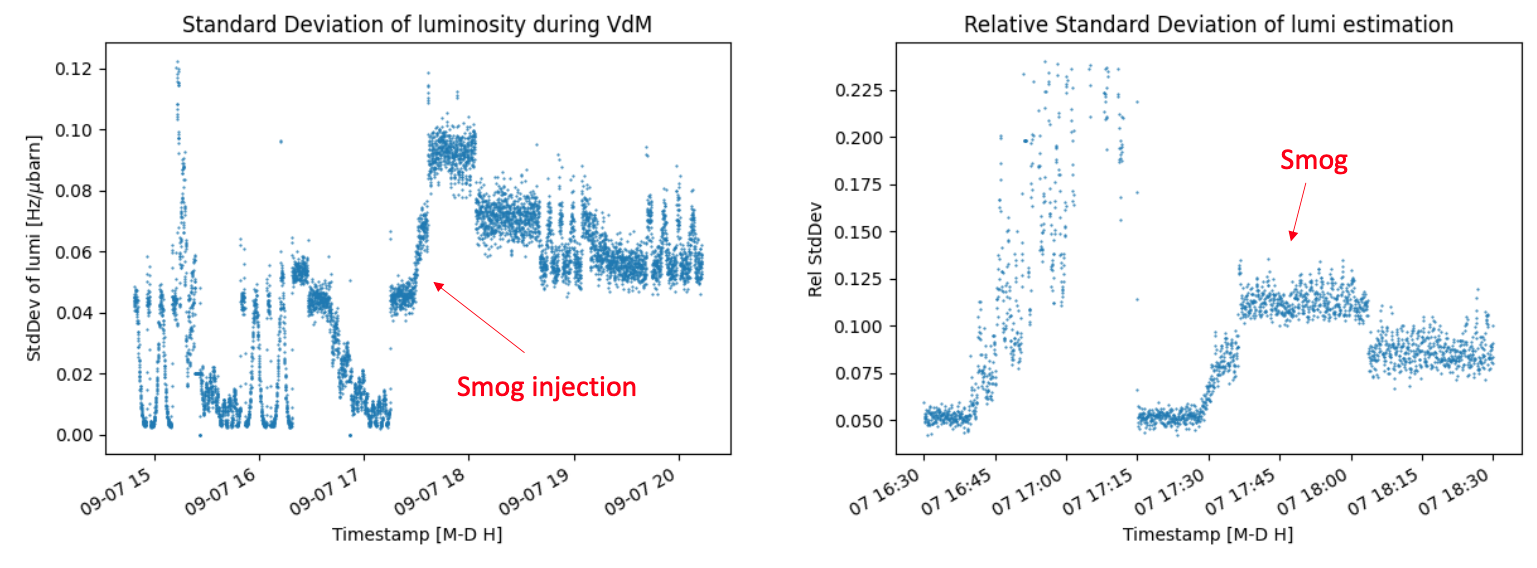
\includegraphics[width=\textwidth]{figures/std_dev_and_rel_std.png}
    \caption{Standard deviation (left) and relative standard deviation (right) of the luminosity estimators during the VdM fill. Notice how this increase after the injection of SMOG at $\approx$17:40}
    \label{fig:std_dev_rel_std}
\end{figure}


The relative standard deviation $\sigma_{rel}$ is plotted as a function of time in Figure \ref{fig:std_dev_rel_std} (right). One notices that the value is stable at 5\% except for the period where smog is injected in the accelerator (around 17:30) and for the time where the mean value $\mu$ of the luminosity is approximately zero (between 16:45 and 17:15).  

This study assures us that the calibration is stable in the short-time term, and that all the counters provide a reasonable luminosity measurement. However, when combining a large set of measurements, it's critical to choose an appropriate estimator to ensure that the final result is reliable and robust. With a dataset containing 208 individual measurements, the presence of outliers or deviations from the assumed probability distribution cannot be excluded. Consequently, choosing a robust estimator becomes essential to mitigate the impact of such anomalies.

Robustness in statistics refers to the ability of an estimator to resist the influence of outliers and remain relatively stable under deviations from standard assumptions. A robust estimator doesn't significantly change due to a small number of atypical values or when the distribution deviates from a presumed normality.

In this context, I tested the performance of three different estimators to determine the best approach for combining my measurements: the mean, the median, and the trimmed mean. Each estimator has its strengths and weaknesses in terms of robustness.

\begin{itemize}
\item Mean: The mean is a common estimator, but it's highly sensitive to outliers. Even a single extreme value can significantly skew the result, making it less suitable for datasets with potential anomalies.
\item Median: The median, which represents the middle value in a dataset, is inherently robust because it is not influenced by outliers. It's often used when the data distribution is skewed or when outliers are present.
\item Trimmed Mean: The trimmed mean is a compromise between the mean and the median. It involves removing a specified percentage of the largest and smallest values from the dataset before calculating the mean. This approach retains some of the data's central tendency while reducing the effect of extreme values.
\end{itemize}


An overview of the behaviour of these three estimators during the VdM is plotted in Figure \ref{fig:lumi_estimator_location_param}. By eye, the behaviour of the three estimators in Figure \ref{fig:comparison_whole} is very similar to one another. However, in a zoomed region such as the one in Figure \ref{fig:comparison_zoom} one can notice how sudden drops in luminosity are differently registered by each one of the tested estimator. Otherwise, the behaviour of these three estimators does not really change.
 

\begin{figure}
    \centering
    \begin{subfigure}{0.48\textwidth}
    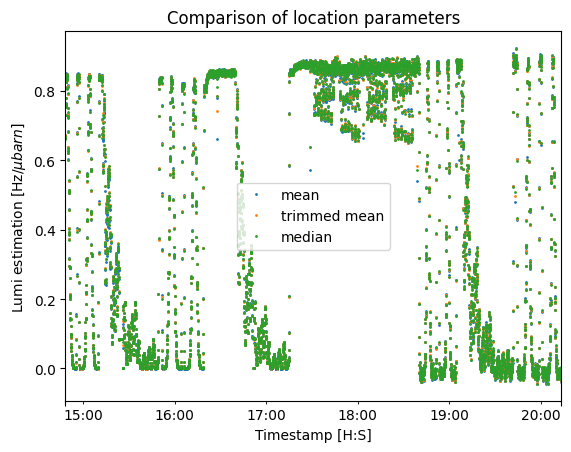
\includegraphics[width=\linewidth]{figures/comparison_location_whole.png}
    \caption{Whole fill}\label{fig:comparison_whole}
    \end{subfigure}
    \begin{subfigure}{0.48\textwidth}
    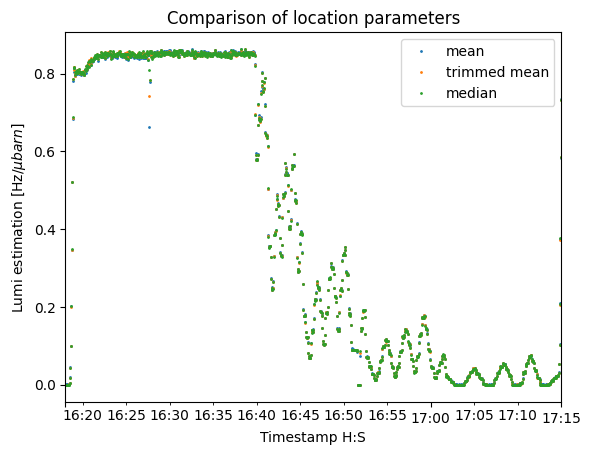
\includegraphics[width=\linewidth]{figures/comparison_location.png}
    \caption{Zoom on constant region and 2D scan}\label{fig:comparison_zoom}
    \end{subfigure}
    \caption{Comparison of three possible location parameter over the VdM Fill. In green: median, in blue: mean, in orange: trimmed mean (15\%)}
    \label{fig:lumi_estimator_location_param}
\end{figure}

In order to test the performances of these estimators, I selected a region during the VdM scan where the luminosity should be constant in time. Then, I fitted an horizontal line (Figure \ref{fig:costant_fit_location}) and computed the residuals of each estimator with respect to the fitted constant. By observing the standard deviation of the distribution of the residuals shown in Figure \ref{fig:res_location}, we can evaluate the precision in time of each estimators. Each one performed similarly, yielding a luminosity resolution of 0.5\% every 3 seconds of data taking.

Based on my initial tests, I found that the median and the trimmed mean were more robust estimators compared to the mean. Given the potential for outliers and the uncertainty in the underlying probability distribution, I selected the trimmed mean at 15\% as the most appropriate estimator for my final analysis. It provides a balance between the stability of the median and the information content of the mean, ensuring a reliable estimate while minimizing the influence of outliers.

\begin{figure}
    \centering
    \begin{subfigure}{0.48\textwidth}
    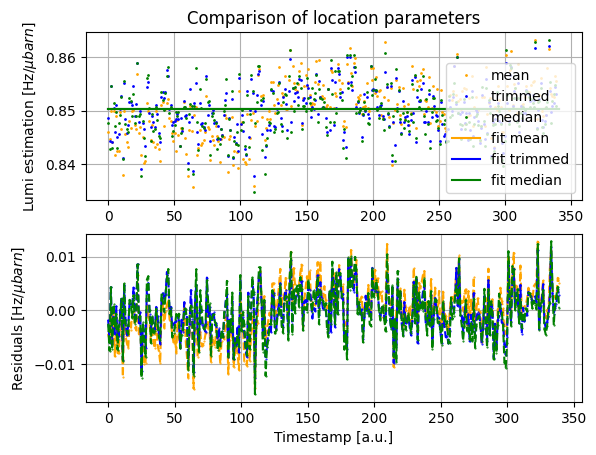
\includegraphics[width=\linewidth]{figures/fit_wo_outliers.png}
    \caption{Constant fit}\label{fig:costant_fit_location}
    \end{subfigure}
    \begin{subfigure}{0.48\textwidth}
    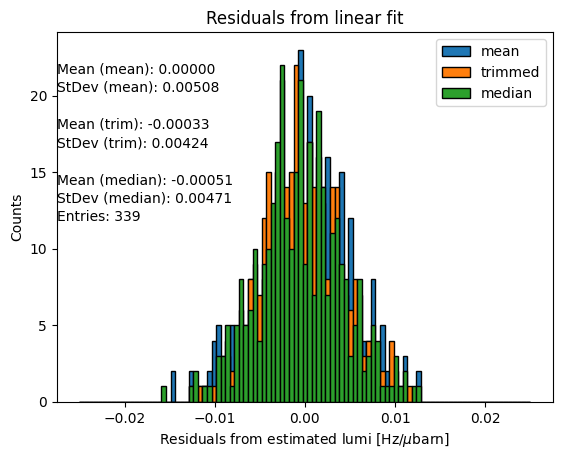
\includegraphics[width=\linewidth]{figures/resiudals_without_outliers.png}
    \caption{Residuals}\label{fig:res_location}
    \end{subfigure}
    \caption{Comparison of three possible location parameter over a stable region of luminosity}
    \label{fig:lumi_fit_location_param}
\end{figure}

The results of my estimator defined as the trimmed mean of the various luminosity measurement performed by each counter is depicted as a function of time during the VdM scan in the second panel of Figure \ref{fig:lumi_result_all}. 

Figure \ref{fig:lumi_result_all} provide a good summary of my analysis of this VdM scan. In the first panel the average counts of each counter is reported, with its background subtracted, while on the third and fourth panel the movements of the two beams respectively in the x and y direction are depicted.

\begin{figure}
    \centering
    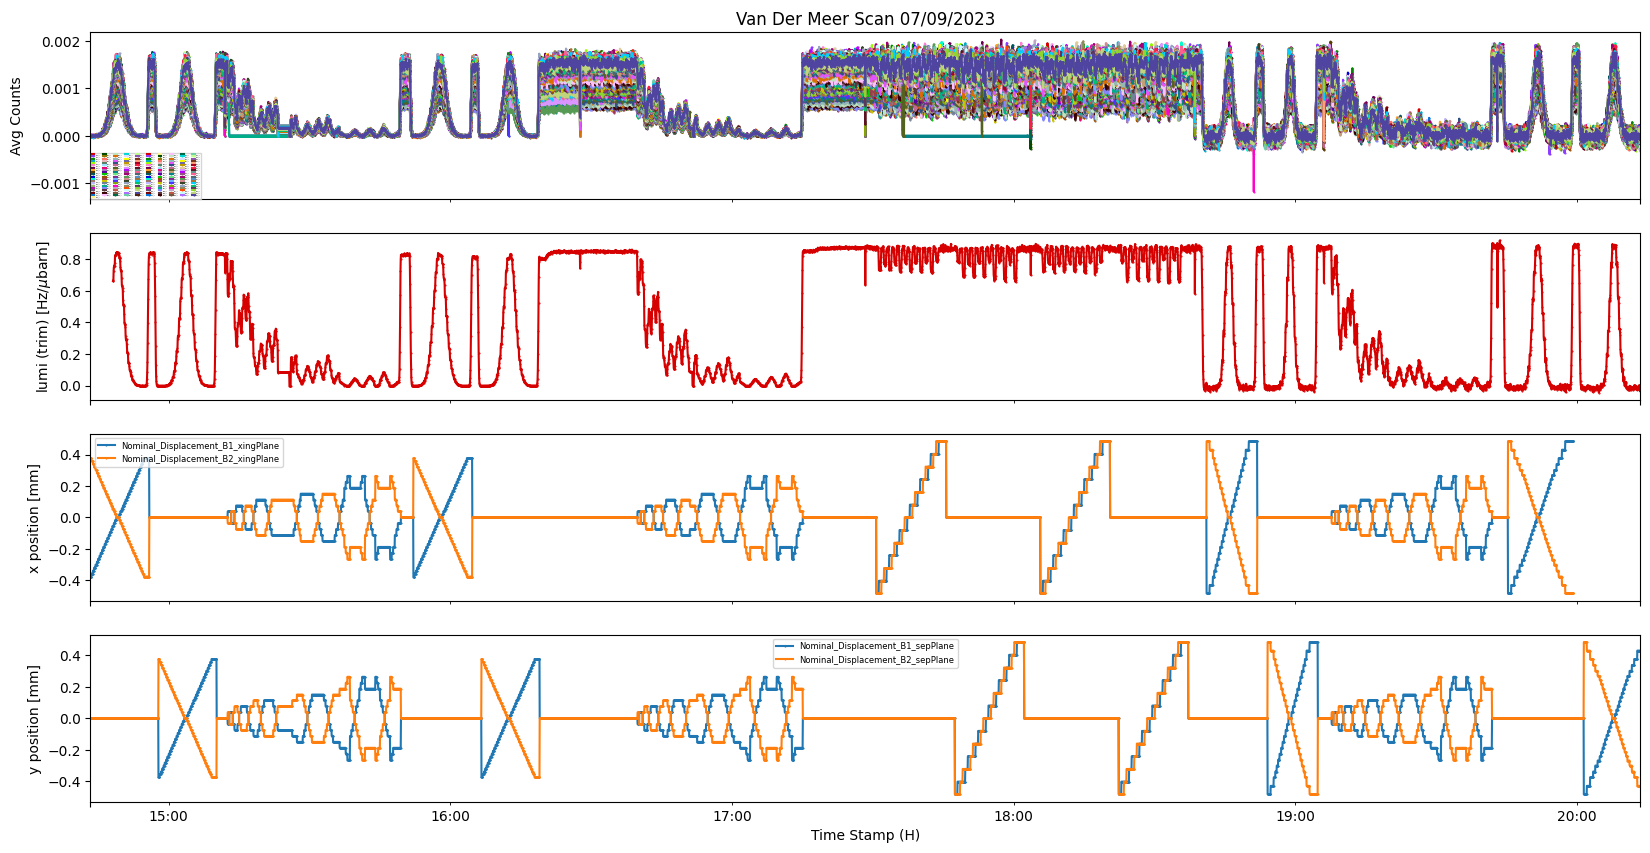
\includegraphics[width=\textwidth]{figures/lumi_plot.png}
    \caption{Results of the luminosity estimator [second panel] during the VdM scan conducted on 07/09/23.
The first panel illustrates the raw mean counts per event of the 208 counters, while the third and fourth
panels respectively depict the x and y positions of the two beams.}
    \label{fig:lumi_result_all}
\end{figure}


To evaluate the medium-term stability of the calibration from September 7, 2023, we estimated the luminosity for Fill 9168, which took place on September 17, 2023, during the pp reference run. This estimation used the visible cross-section $\sigma_{vis}$ derived from the VdM scan. Figure \ref{fig:fill9168} provides an overview of the results from this study.

In the first panel of Figure \ref{fig:fill9168}, the luminosity readings from each individual counter are displayed. Unfortunately, during this fill, only the C side of the VELO was operational, reducing our available data and resulting in a significant drop in statistics. The second panel shows the combined luminosity estimate, calculated as the trimmed mean of the functional counters. The third panel displays the relative standard deviation of the luminosity measurements for each counter. As seen in the figure, the relative standard deviation stabilizes at around 3\%, which is reasonably close to the 5\% observed during the VdM scan, considering that the statistics were effectively halved.

Despite the reduced data due to limited VELO operation, the relative stability of the combined luminosity estimate indicates that the calibration from the earlier VdM scan remains reliable in the medium term. The consistency of the relative standard deviation suggests that the estimation method is robust, even with reduced sample sizes, providing confidence in the calibration's effectiveness across different datasets and time periods.


\begin{figure}
    \centering
    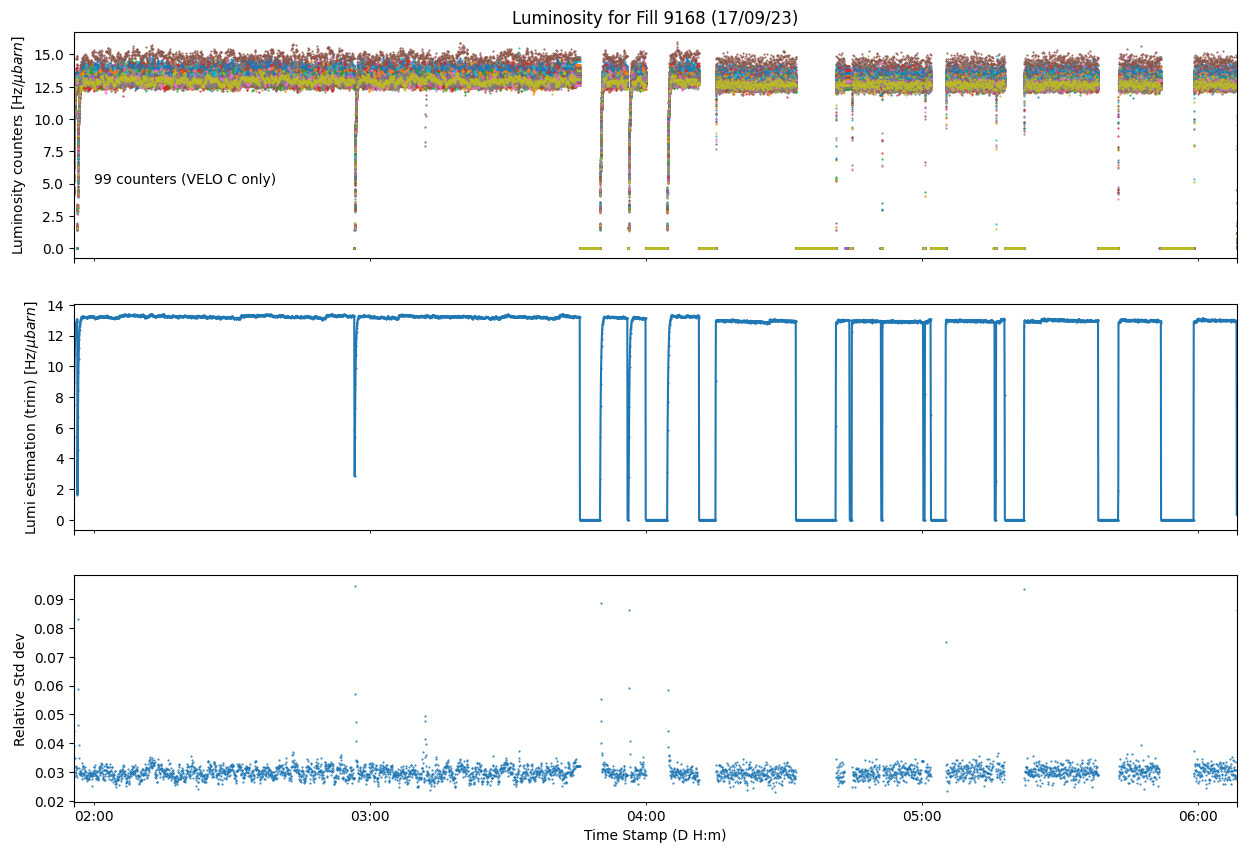
\includegraphics[width=\textwidth]{figures/fill9168.png}
    \caption{Luminosity during pp reference Run - Fill 9168.}
    \label{fig:fill9168}
\end{figure}